\documentclass[UTF8,a4paper]{ctexart}
\usepackage[utf8]{inputenc}
\usepackage{amsmath}
\usepackage{pdfpages}
\usepackage{graphicx}
\usepackage{wrapfig}
\usepackage{listings}
\usepackage{multicol}
\newcommand{\tabincell}[2]{\begin{tabular}{@{}#1@{}}#2\end{tabular}}
\title{实验一\ \ 单管放大电路仿真及实验}
\author{张蔚桐\ 2015011493\ 自55}
\begin {document}
\maketitle
\section{预习任务(仿真部分)}
\subsection{电路放大原理}
\begin {wrapfigure}{r}{0pt}
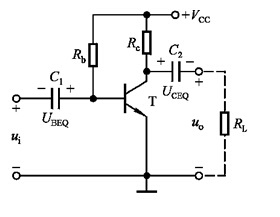
\includegraphics [width=40mm]{basic.jpg}
\caption{基本阻容耦合电路图}
\label{basic}
\end {wrapfigure}
以阻容耦合电路为例,如图\ref{basic}所示,集电极电源$V_{CC}$ 通过基极电阻$R_b$ 和集电极电阻$R_c$ 提供合适的$U_{be}$ 和$U_{ce}$,使晶体管处于放大区。为了保证放大电路正常工作,需要通过调整参数得到合适的静态工作点,保证输入信号在一定范围内时最终的信号不会失真。有交流小信号$u_i$ 作用时,交流量驼载在直流量上。输入信号通过容抗很小的电容加在发射结上,小电流经过晶体管放大后,在集电极产生放大的电流,通过$R_c$ 转换为电压变化,从而实现了对动态电压信号的放大。
\subsection{理论预估}
\begin {wrapfigure}{r}{0pt}
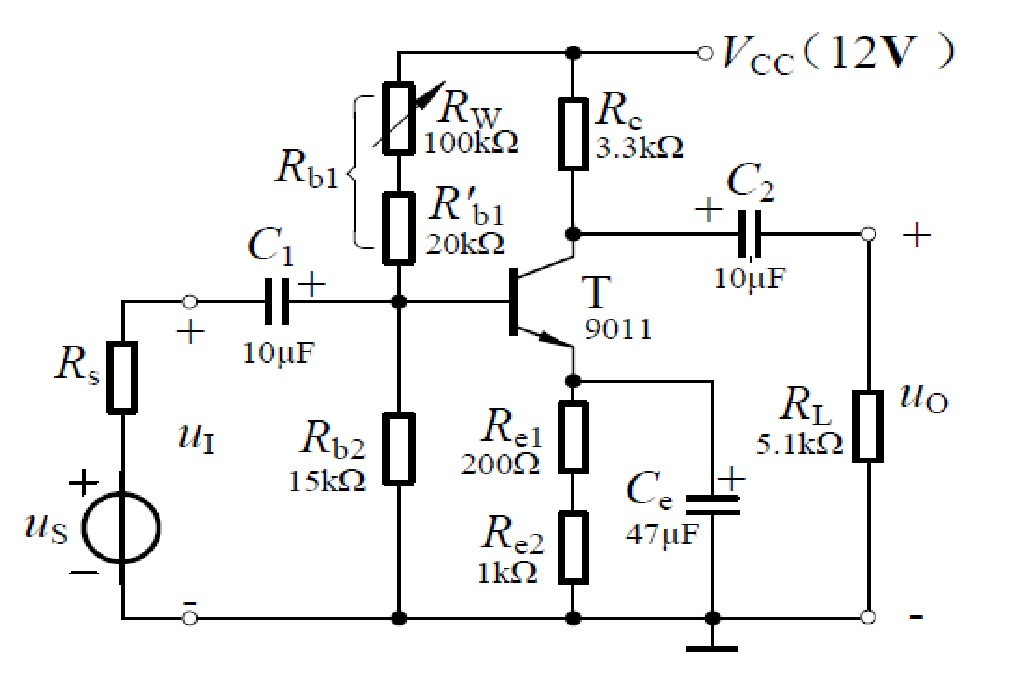
\includegraphics [width=55mm]{circuit.jpg}
\caption{单管共射放大电路}
\label{circuit}
\end {wrapfigure}
如图\ref{circuit}所示是实验用电路图,其中进行理论估算时取$r_{bb'}=100\Omega$于是可得$r_{be}=r_{bb'}+\frac{U_T}{I_{BQ}}\approx100\Omega+\frac{26\rm{mV}}{10\rm{\mu A}}\approx1\rm{k}$$\Omega$其中上式的各项参数按照经典值进行估计,$\beta$估计为100。需要注意的是,上面所有的估计仅为在数量级上的估计。同样可以简单预估得到$R_i\approx1k\Omega,R_o\approx3.3k\Omega,\dot{A}=-\frac{\beta R_L'}{r_{be}}\approx-30$ 上面对数量级的简单估计有助于进一步调试的时候对电阻的选取

\subsection{EDA中对$\beta$的测量} 
\begin {wrapfigure}{r}{0pt}
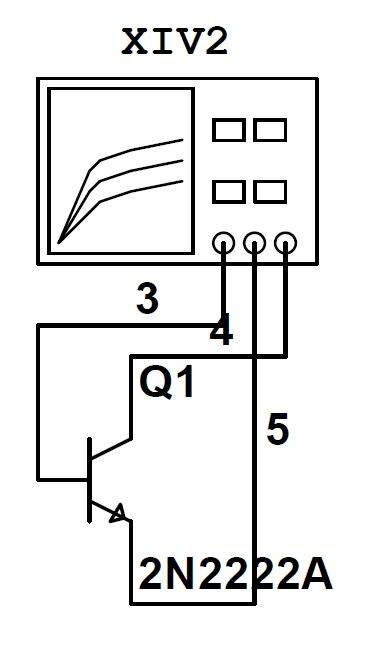
\includegraphics [width=20mm]{9.JPG}
\caption{晶体管$\beta$测试电路图}
\label{TCirc}
\end {wrapfigure}
采用如图\ref{TCirc}的电路进行测试,将晶体管按照IV测试仪的指示接入IV测试仪,将“Component”设置为“BJT NPN”,将$I_b$设置为$0\rm{A} -- 10\rm{\mu A} $,$U_{ce}$设置为0V~10V进行宽范围测试,得到图\ref{Tgeneral}所示的结果 
\begin {figure}
\centering
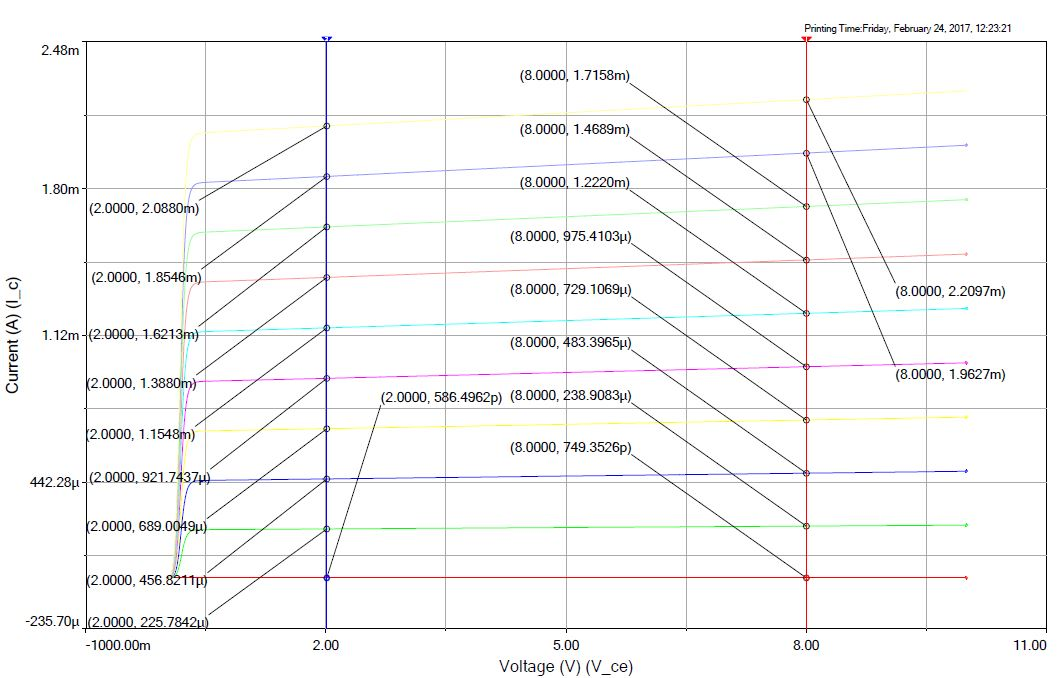
\includegraphics[width=\textwidth]{17.JPG}
\caption{晶体管输出特性}
\label{Tgeneral}
\end{figure}
在图\ref{Tgeneral}中标识了在$U_{ce}=2\rm{V}$和$U_{ce}=8\rm{V}$下,$I_c$随着$I_b$的变化情况,具体来说可以总结为下表
\\
\begin{table}
\centering
\caption{对$\beta$的仿真}
\label{b_simu}
\begin{tabular}{|c|c|c|}
\hline
\tabincell{c}{$I_b/\rm{\mu A}$}& \tabincell{c}{$I_c/\rm{mA}@U_{ce}=2\rm{V}$}& \tabincell{c}{$I_c/\rm{mA}@U_{ce}=8\rm{V}$}\\
\hline
0.00&0.0005&0.0007 \\
\hline
1.11&0.2258 &0.2389 \\
\hline
2.22&0.4568 &0.4834 \\
\hline
3.33&0.6890 &0.7291 \\
\hline
4.44&0.9217 &0.9754 \\
\hline
5.56&1.1549 &1.2220 \\
\hline
6.67&1.3880 &1.4689 \\
\hline
7.78&1.6213 &1.7158 \\
\hline
8.89&1.8546 &1.9627 \\
\hline
10&2.0880 &2.2097 \\
\hline
\end{tabular}
\end{table}
\\

于是可以对两种情况下的$I_c$和$I_b$做直线拟合得到
$$I_c=209.06I_b-5.2456(\rm{\mu A})@U_{ce}=2\rm{V},R^2=1,\beta=209.06$$
$$I_c=221.24I_b-5.5308(\rm{\mu A})@U_{ce}=8\rm{V},R^2=1,\beta=221.24$$

因此可以认为晶体管的$\beta=215$
\subsection{理论计算}
根据相关知识,可以得到在实验参考值$I_{CQ}=1\rm{mA}$或$I_{CQ}=2\rm{mA}$时的相关参数$\dot{A}_u,R_o,R_i$
\subsubsection{$I_{CQ}=1\rm{mA}$时}
此时有,$I_{BQ}=\frac{I_{CQ}}{\beta}=4.65\rm{\mu A},I_{EQ}=\frac{(1+\beta)I_{CQ}}{\beta}=1\rm{mA}$ 并进一步得到$U_{EQ}=1.2\rm{V},U_{BQ}=U_{EQ}+U_{BEQ}=1.2+0.7=1.9\rm{V}$,于是可以估计$R_{b1}=\frac{V_{CC}-U_{BQ}}{U_{BQ}}R_{b2}=\frac{10.1}{1.9}\times15\rm{k}$$\Omega=79\rm{k}$$\Omega$并进一步得到$R_W=59\rm{k}$$\Omega$$,U_{CQ}=8.7\rm{V}$

经过进一步的计算,可以得到$R_o=3.3\rm{k}$$\Omega$,$r_{be}=100\Omega+\frac{26\rm{mV}}{4.65\rm{\mu A}}=5.7k$$\Omega,R_i=r_{be}//R_{b2}//R_{b1}=3.9k$$\Omega,\dot{A}_u=\frac{\beta(R_o//R_L)}{r_{be}}=75.57$发现和前文的数量级估算是符合的。
\subsubsection{$I_{CQ}=2\rm{mA}$时}
此时同上节重新计算,得到$I_{BQ}=9.30\rm{\mu A},I_{EQ}=2\rm{mA},U_{EQ}=2.4\rm{V},U_{BQ}=3.1\rm{V},R_{b1}=43\rm{k}$$\Omega,R_W=23\rm{k}$$\Omega,R_o=3.3\rm{k}$$\Omega$,$r_{be}=2.9k$$\Omega,R_i=2.3k$$\Omega,\dot{A}_u=148.5,U_{CQ}=5.4\rm{V}$发现和前文的数量级估算是符合的。
\subsection{仿真测试}
\subsubsection{静态工作点测试}
如图\ref{circuit}在Multisim上搭建电路,将交流源置零,调整$R_W$直到$I_{CQ}=1\rm{mA}$以及$I_{CQ}=2\rm{mA}$,得到如图\ref{1}和图\ref{2}的电路静态工作点参数
因此得到,$I_{CQ}=1\rm{mA}$时,$U_{CQ}=8.69\rm{V},U_{EQ}=1.21\rm{V},U_{CEQ}=7.48\rm{V},R_W=60k$$\Omega$

因此得到,$I_{CQ}=2\rm{mA}$时,$U_{CQ}=5.41\rm{V},U_{EQ}=2.41\rm{V},U_{CEQ}=3.00\rm{V},R_W=22k$$\Omega$

和之前计算的结果的误差均在仿真采用的分度值之内,可以忽略。

\subsubsection{动态工作点测试}
将交流源设置为$V_{pp}=20\rm{mV},f=10kHz$的正弦信号,进行测试,针对$I_{CQ}=1\rm{mA}$和$I_{CQ}=2\rm{mA}$时,按照题目要求经过仿真测试可得如下结果,其中前两个情况的bode图如图\ref{bode1}\ref{bode2}所示。可以看出,和理论计算情况基本相符。
\\
\begin{table}
\centering
\caption{仿真实验结果}
\label{simu}
\begin{tabular}{|c|c|c|c|c|c|c|c|}
\hline
\tabincell{c}{$I_{CQ}/\rm{mA}$}& \tabincell{c}{$\dot{A}_u$}& \tabincell{c}{$R_i/\rm{k}$$\Omega$} & \tabincell{c}{无负载\\ $V_{oo}/\rm{mV}$} & \tabincell{c}{$R_0/\rm{k}$$\Omega$}&\tabincell{c}{失真度}&\tabincell{c}{$f_L/kHz$}&\tabincell{c}{$f_H/kHz$}\\
\hline
1.00&74.853&3.88&572.879&3.2&0.04603&0.1346&290\\
\hline
2.00&144.5&2.19&870.245&3.095&0.02686&0.25629&203.4\\
\hline
\tabincell{c}{2.00\\ (射极电阻改变)}&9.3&9.87&85.379&16.72&0.00052&0.0193254&22272\\
\hline
\end{tabular}
\end{table}
\subsubsection{射极电阻对动态特性的影响}
按照实验要求,将电容$C_E$改为与$R_{E2}$并联,测量此时放大电路在静态工作点$I_{CQ}=2\rm{mA}$ 下的$\dot{A}_{u_i}$,实验用电路图显而易见,具体数据记录在上表中
\begin{figure}
\centering
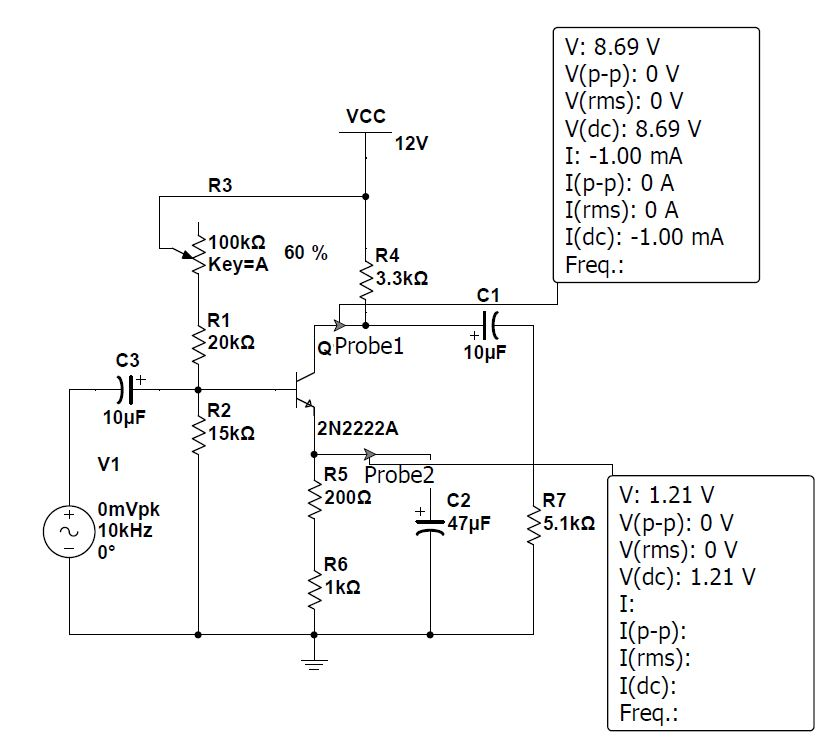
\includegraphics[width=\textwidth]{1.jpg}
\caption{$I_{CQ}=1\rm{mA}$静态参数}
\label{1}
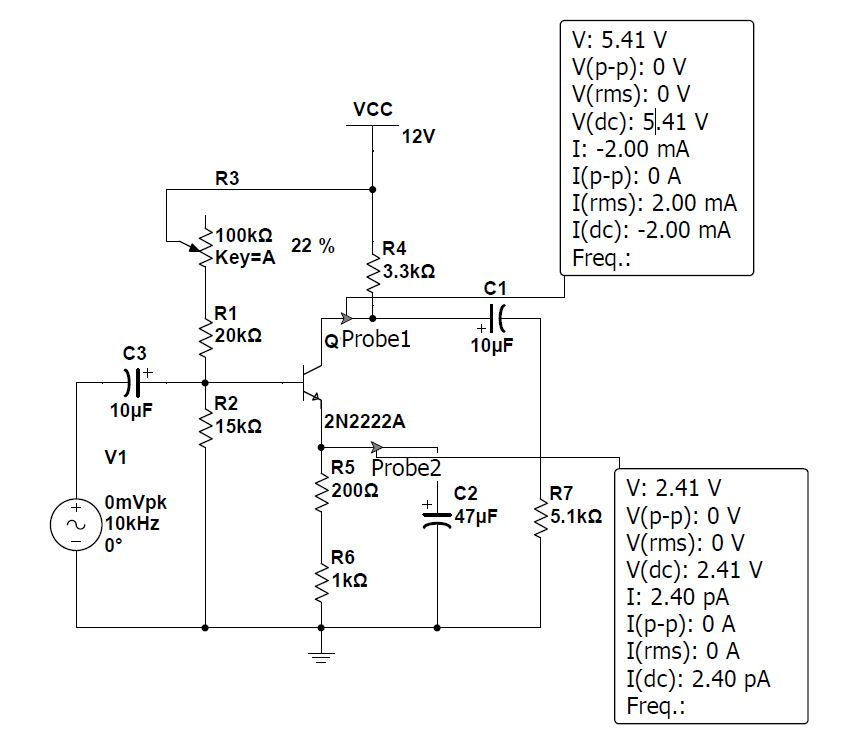
\includegraphics[width=\textwidth]{2.jpg}
\caption{$I_{CQ}=2\rm{mA}$静态参数}
\label{2}
\end{figure}
\begin{figure}
\centering
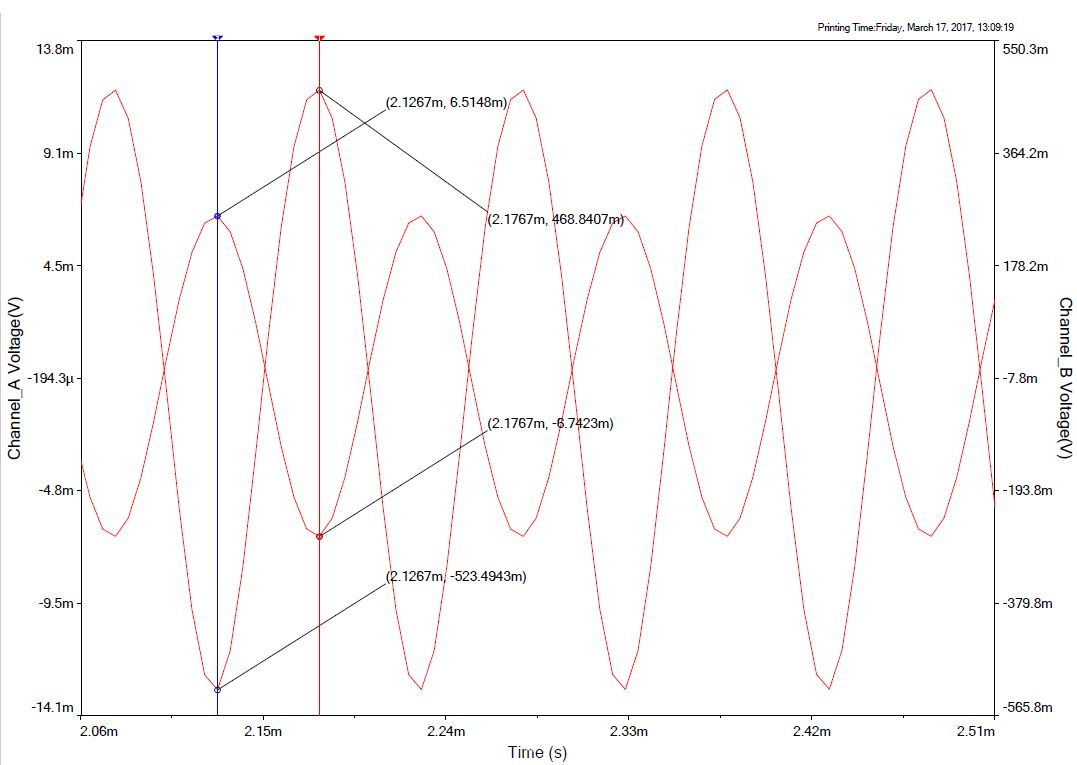
\includegraphics[width=\textwidth]{A1.JPG}
\caption{$I_{CQ}=1\rm{mA}$时的增益情况}
\label{A1}
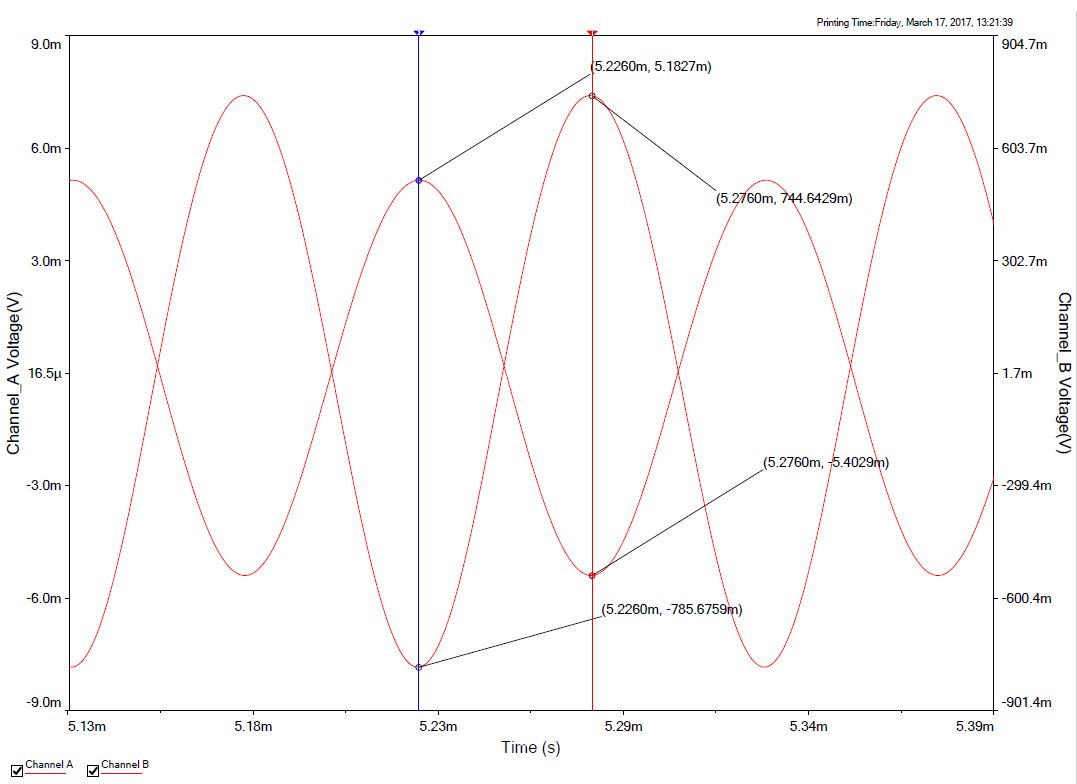
\includegraphics[width=\textwidth]{A2.JPG}
\caption{$I_{CQ}=2\rm{mA}$时的增益情况}
\label{A2}
\end{figure}
\begin{figure}
\centering
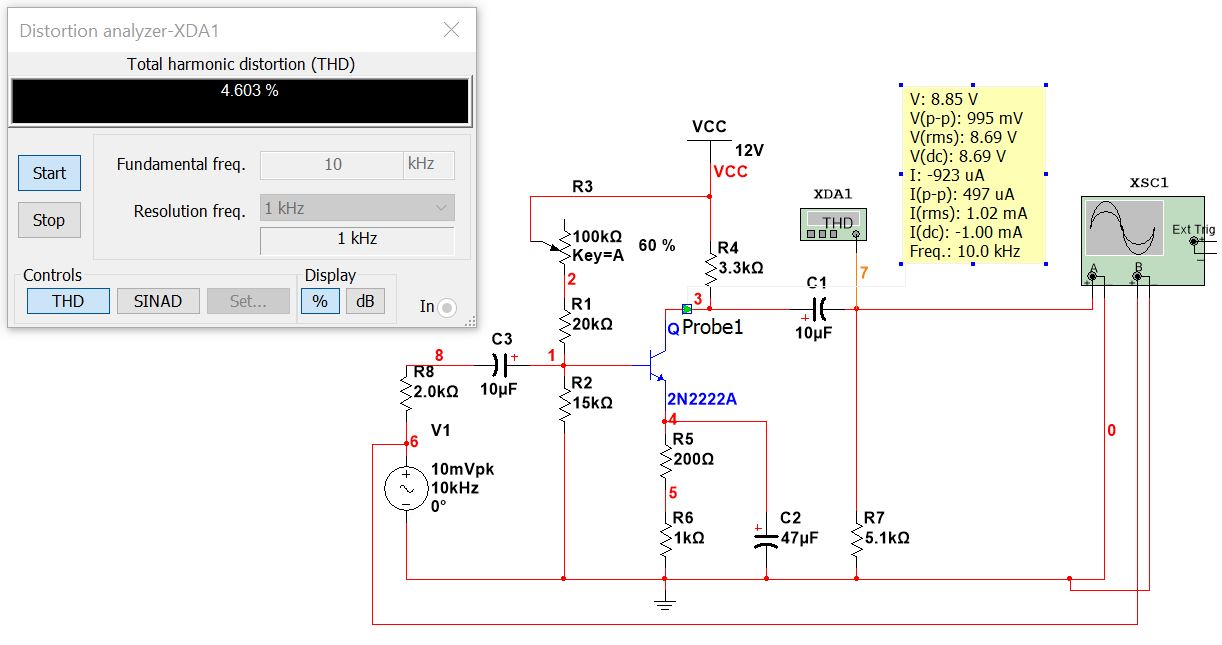
\includegraphics[width=\textwidth]{TI.JPG}
\caption{$I_{CQ}=1\rm{mA}$时的电路仿真图}
\label{C1}
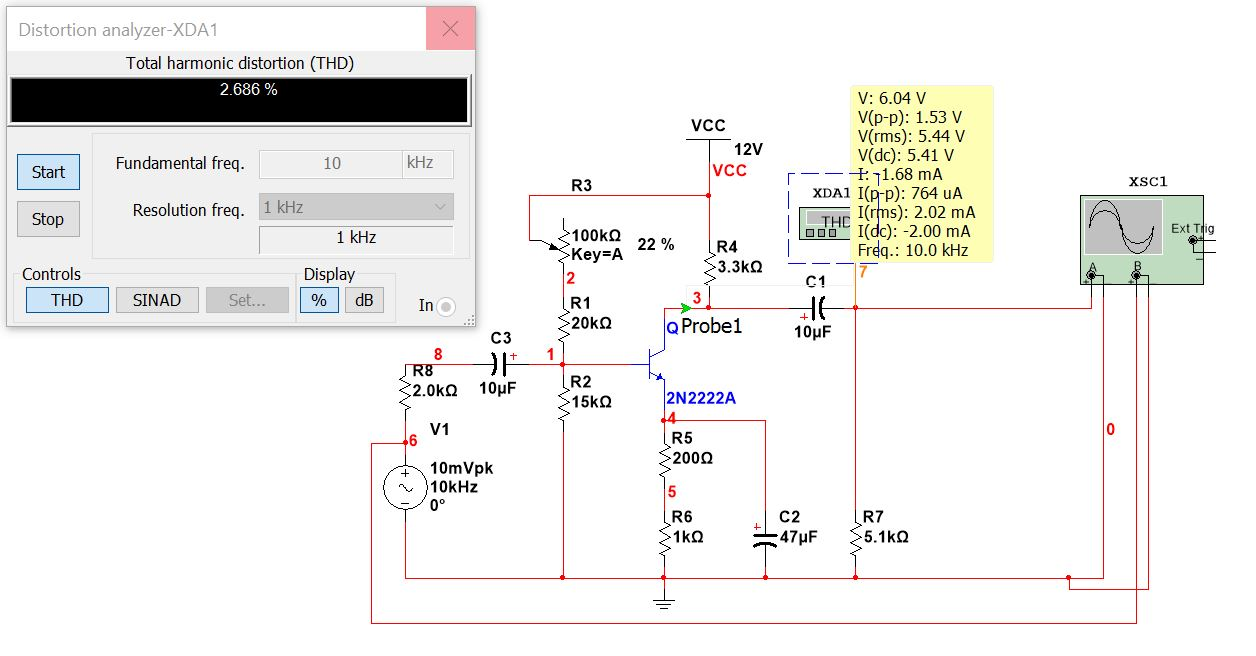
\includegraphics[width=\textwidth]{TII.JPG}
\caption{$I_{CQ}=2\rm{mA}$时的电路仿真图}
\label{C2}
\end{figure}
\begin{figure}
\centering
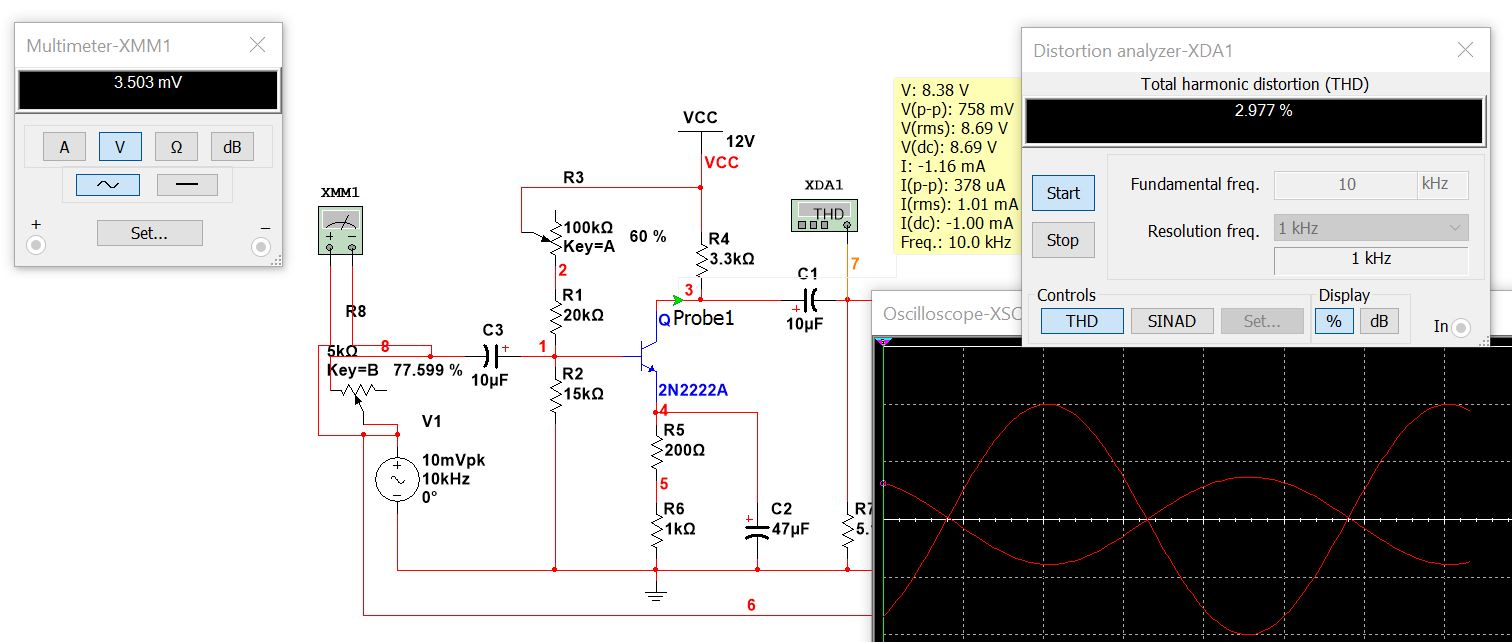
\includegraphics[width=\textwidth]{Ri2.JPG}
\caption{$I_{CQ}=1\rm{mA}$时的$R_i$测量图}
\label{Ri1}
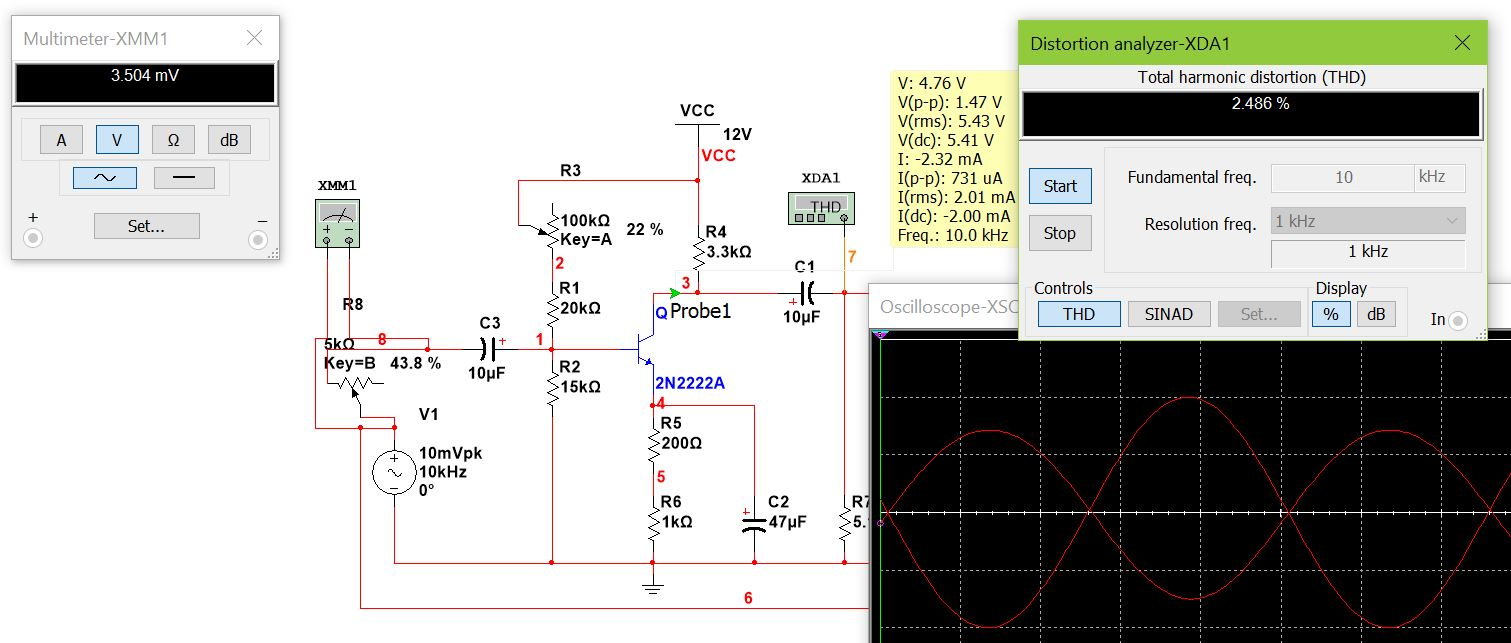
\includegraphics[width=\textwidth]{Ri1.JPG}
\caption{$I_{CQ}=2\rm{mA}$时的$R_i$测量图}
\label{Ri2}
\end{figure}
\begin{figure}
\centering
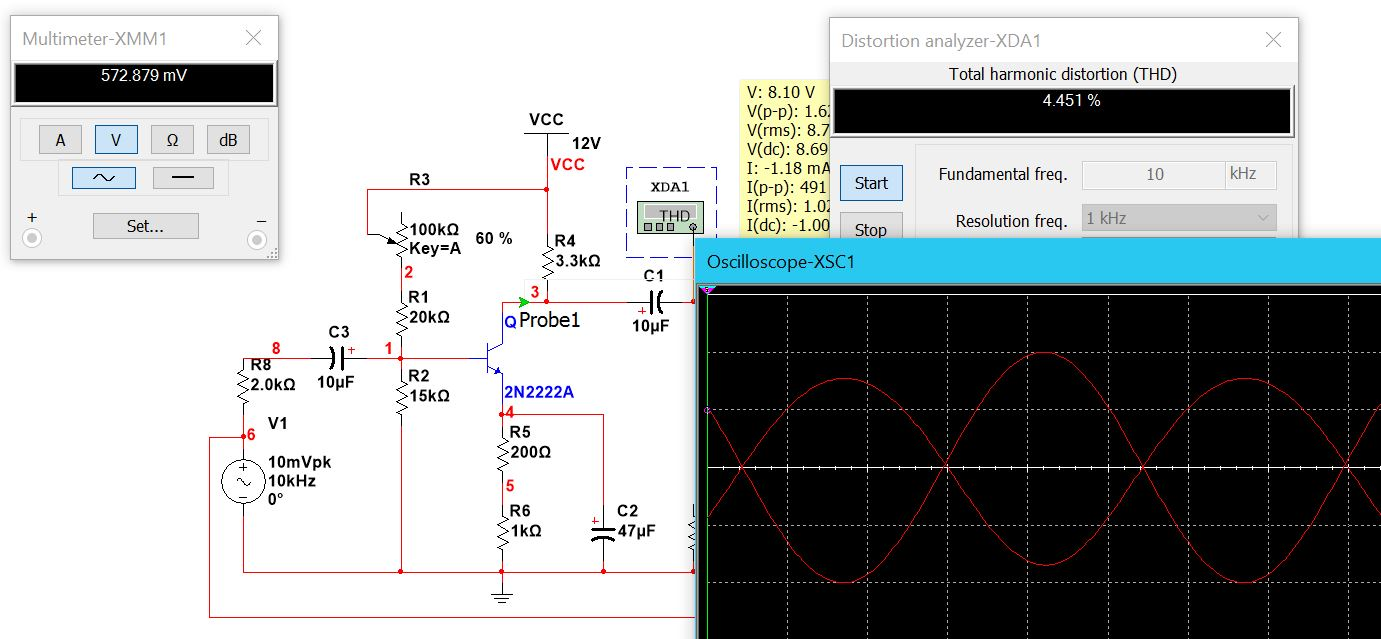
\includegraphics[width=\textwidth]{R02.JPG}
\caption{$I_{CQ}=1\rm{mA}$时的开路电压测量图}
\label{Ri1}
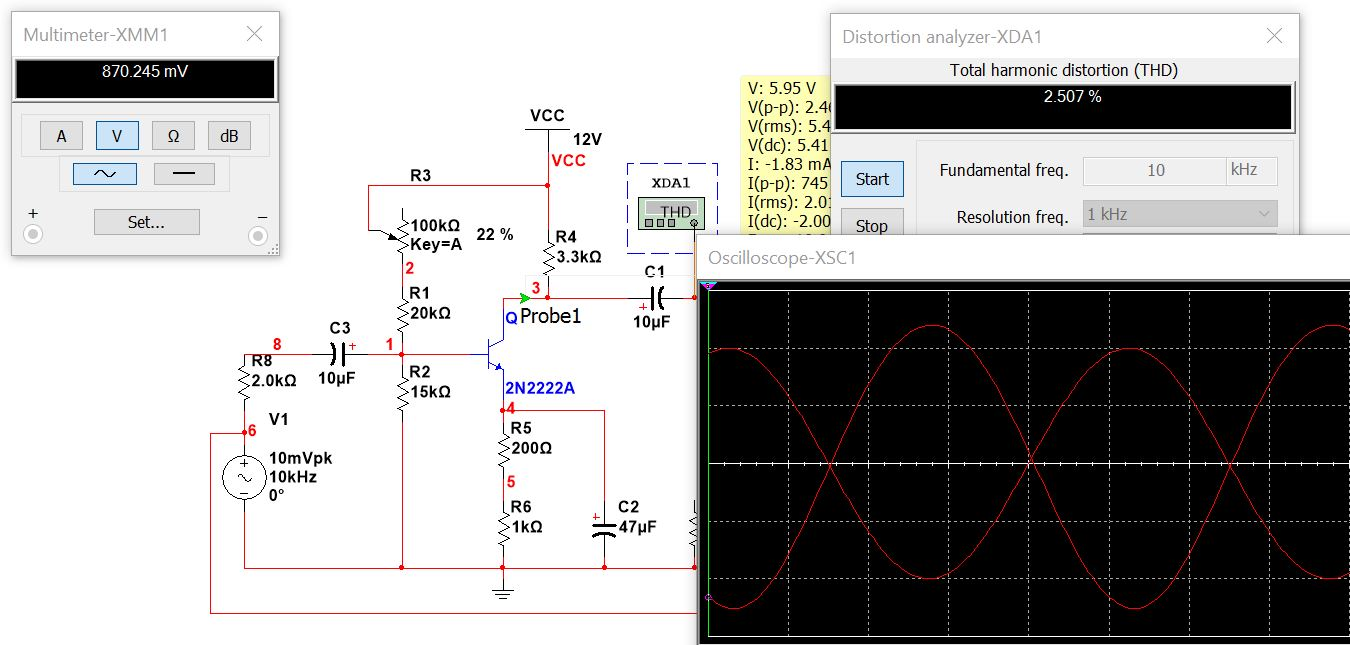
\includegraphics[width=\textwidth]{R01.JPG}
\caption{$I_{CQ}=2\rm{mA}$时的开路电压测量图}
\label{Ri2}
\end{figure}
\begin{figure}
\centering
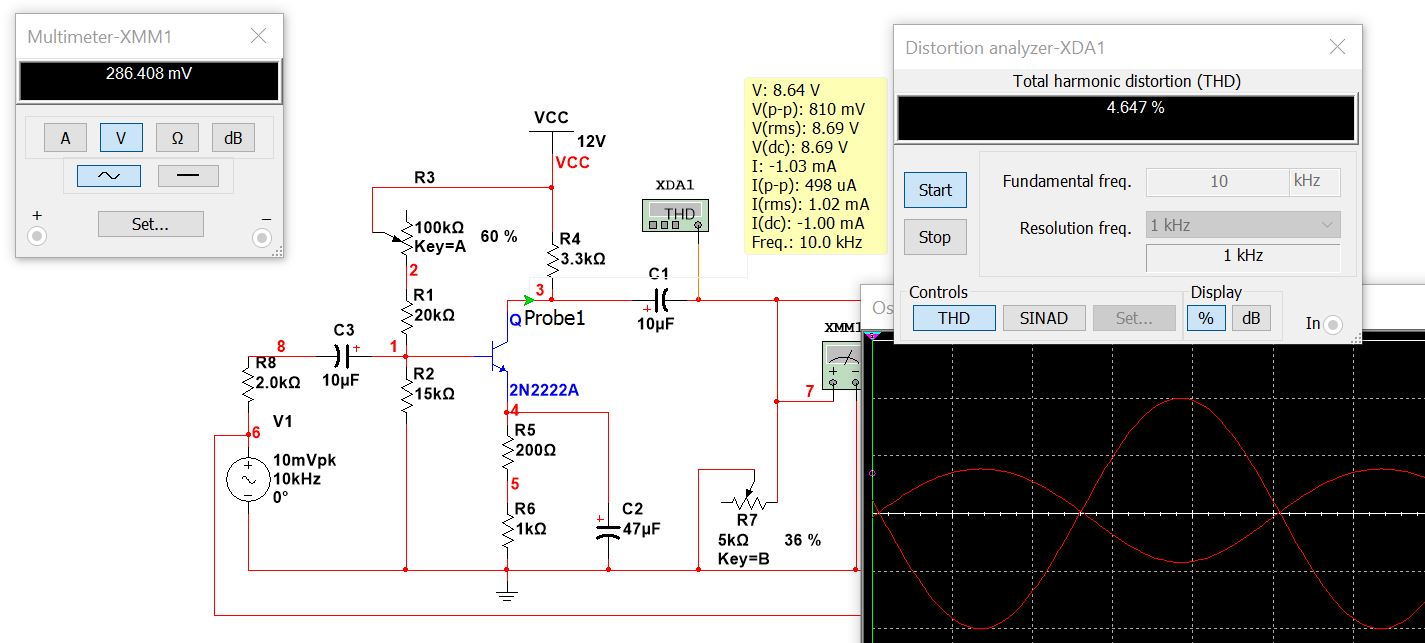
\includegraphics[width=\textwidth]{R002.JPG}
\caption{$I_{CQ}=1\rm{mA}$时的$R_o$测量图}
\label{Ri1}
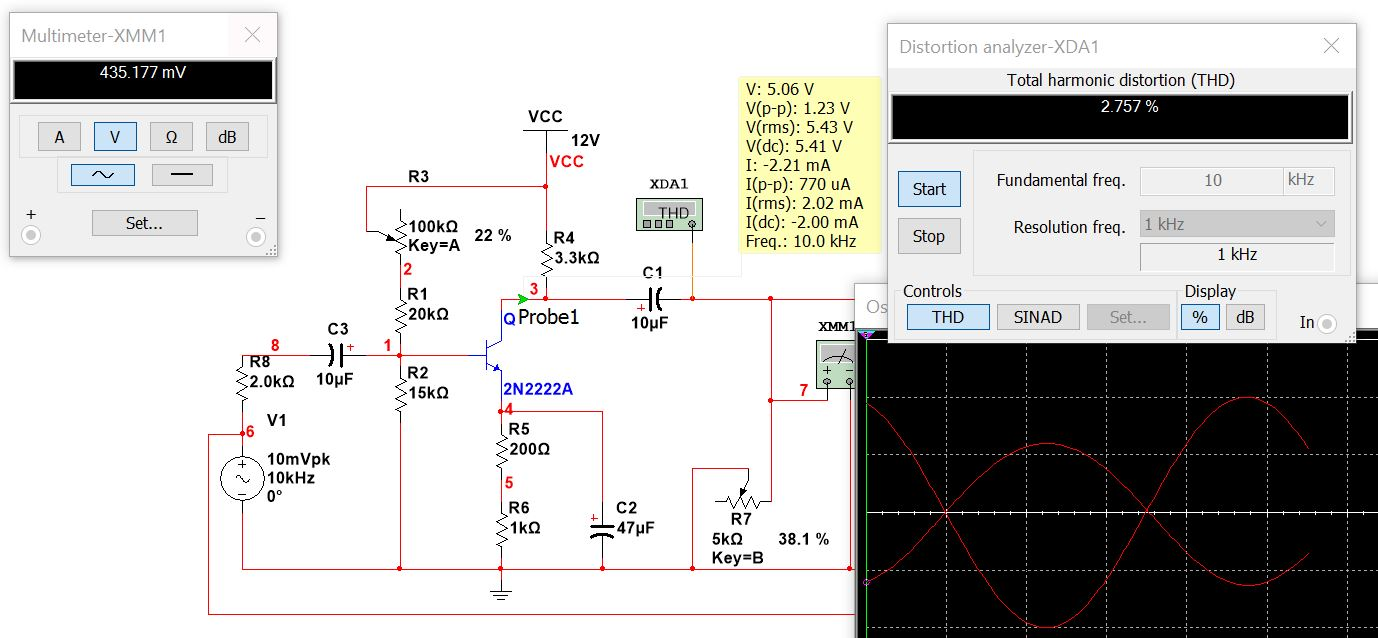
\includegraphics[width=\textwidth]{R001.JPG}
\caption{$I_{CQ}=2\rm{mA}$时的$R_o$测量图}
\label{Ri2}
\end{figure}
\begin{figure}
\centering
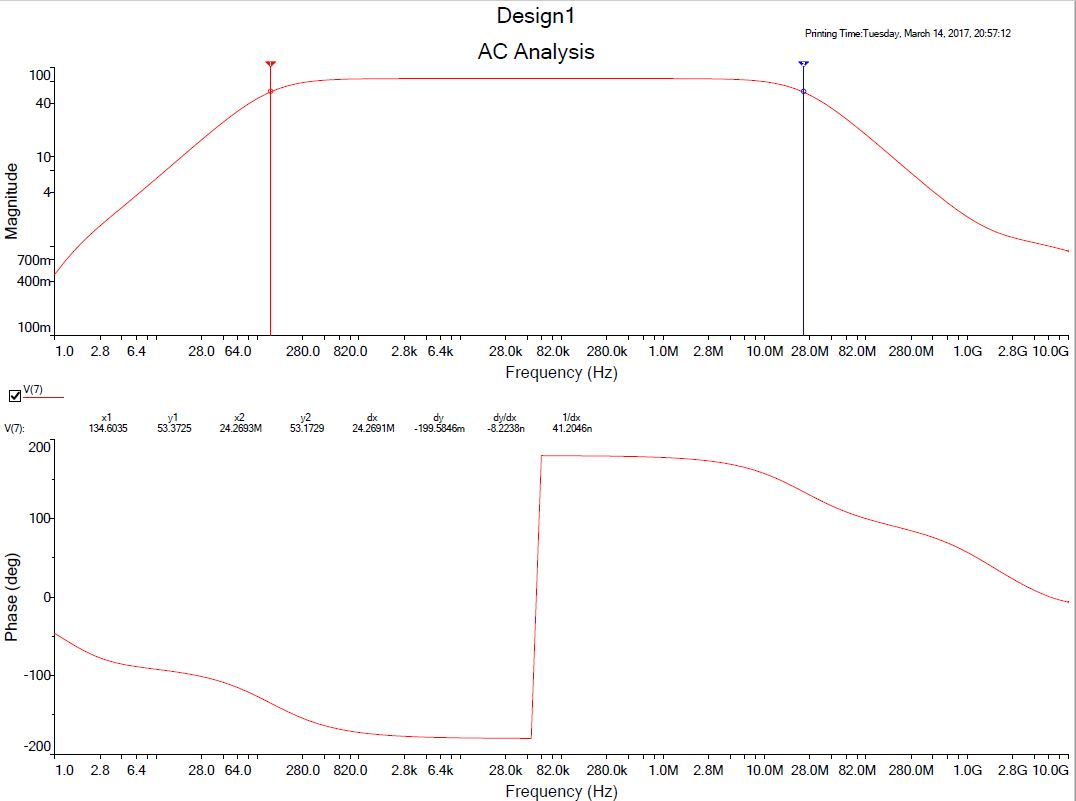
\includegraphics[width=\textwidth]{b1.jpg}
\caption{$I_{CQ}=1\rm{mA}$时的bode图}
\label{bode1}
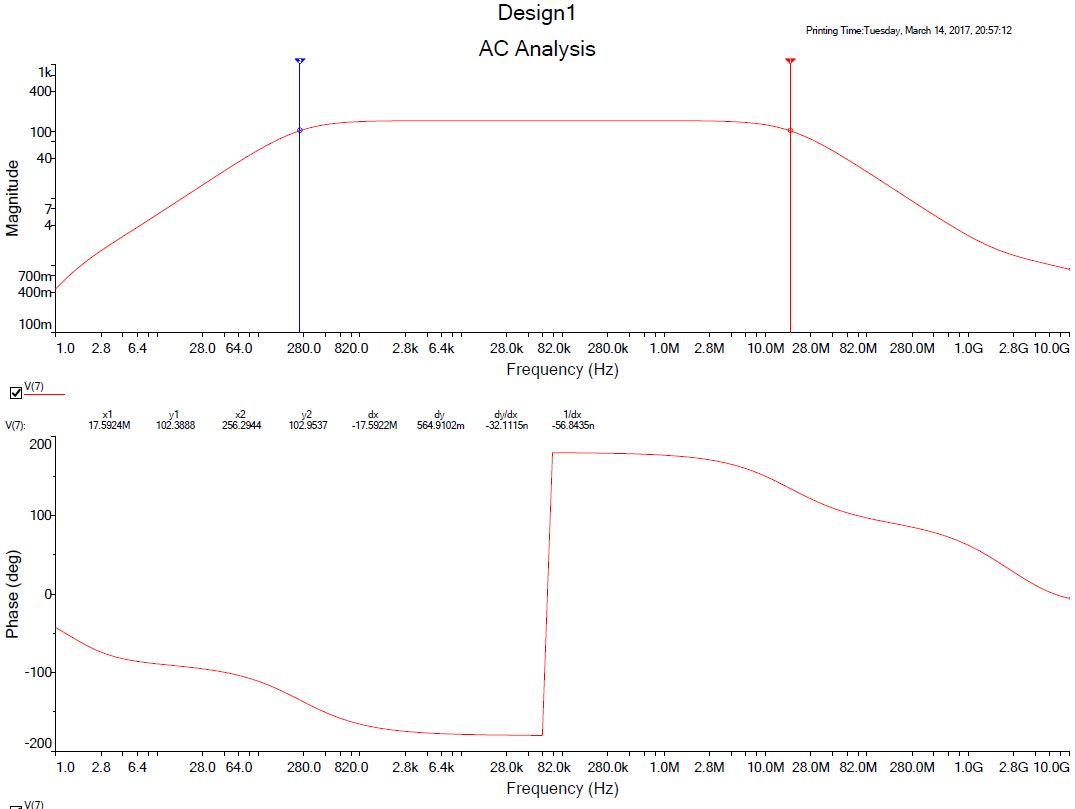
\includegraphics[width=\textwidth]{b2.jpg}
\caption{$I_{CQ}=2\rm{mA}$时的bode图}
\label{bode2}
\end{figure}
\begin{figure}
\centering
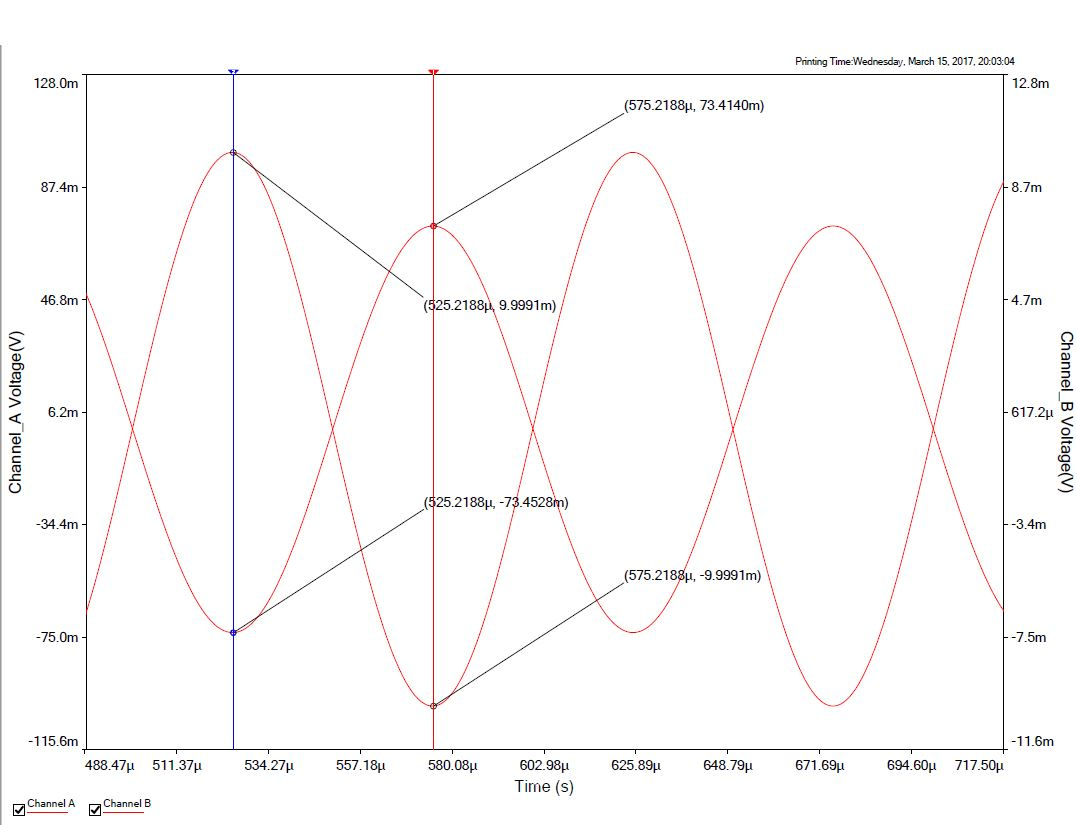
\includegraphics[width=\textwidth]{Capture.JPG}
\caption{$I_{CQ}=2\rm{mA}$,射级电阻改变输入输出波形图}
\label{RE1}
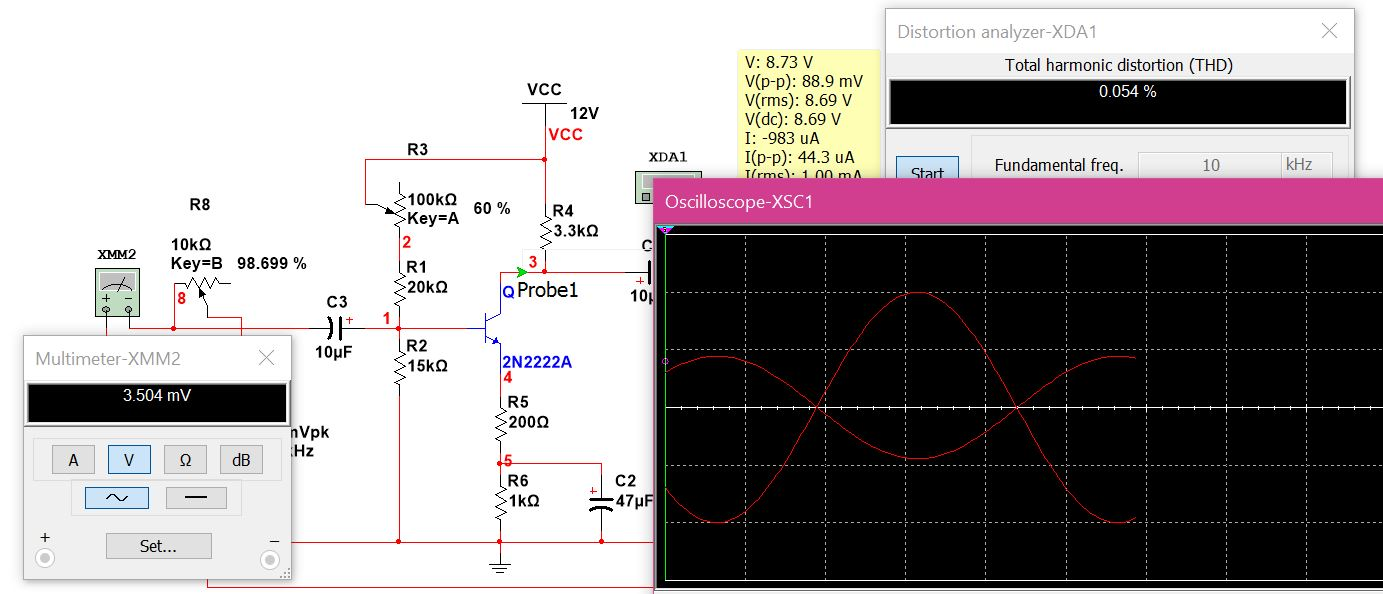
\includegraphics[width=\textwidth]{speri.JPG}
\caption{$I_{CQ}=2\rm{mA}$时的输入电阻测量图}
\label{RERI}
\end{figure}
\begin{figure}
\centering
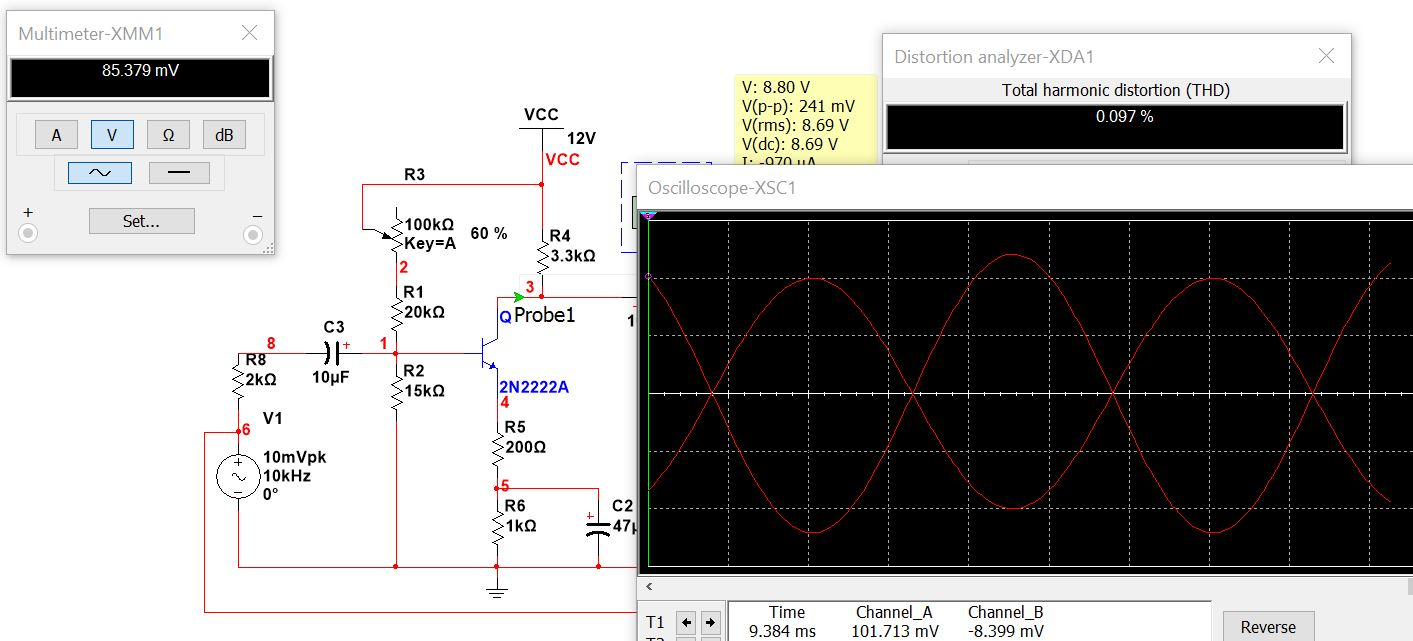
\includegraphics[width=\textwidth]{spero1.JPG}
\caption{$I_{CQ}=2\rm{mA}$时的开路电压测试图}
\label{RERO1}
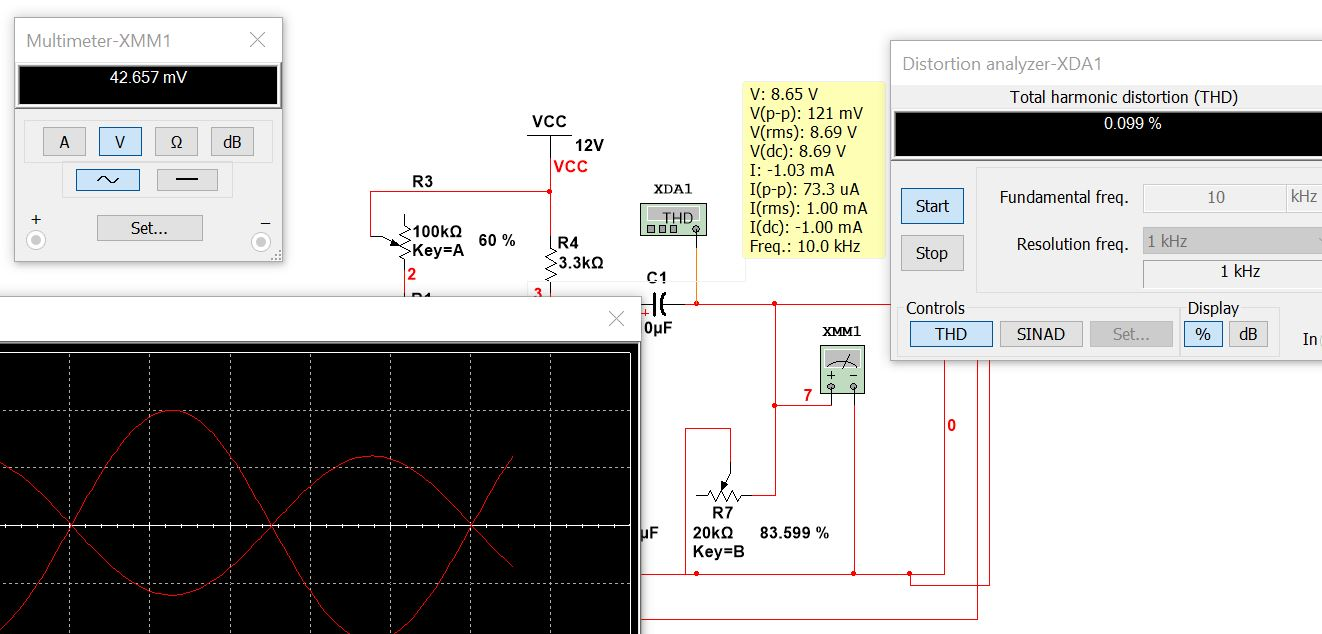
\includegraphics[width=\textwidth]{spero2.JPG}
\caption{$I_{CQ}=2\rm{mA}$时的$R_o$测量图}
\label{RERO2}
\end{figure}
\begin{figure}
\centering
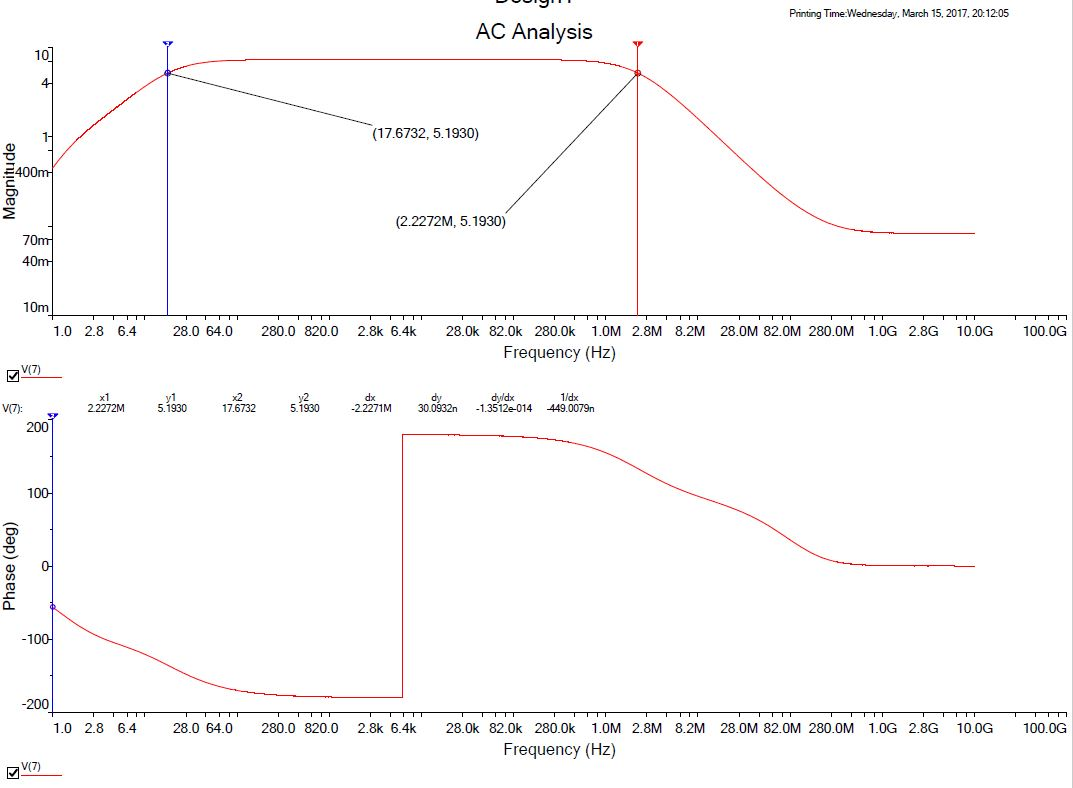
\includegraphics[width=\textwidth]{TB.JPG}
\caption{$I_{CQ}=2\rm{mA}$时的bode图}
\label{REbode}
\end{figure}
\subsection{硬件实验中具体参数的设置方法}
根据电路实验知识和模电相关知识,可以列出可能涉及到的参数的测量方法如下
\subsubsection{静态工作点}
测试静态工作点时,先去掉信号源,并将输入端短路,再用万用表的直流电压档测试。静态电压可用万用表或示波器直接测量,静态电流可通过测量集电极电阻的电压间接测量,避免因为串入电流表带来的误差。
\subsubsection{电压放大倍数}
在输入端加上中频小幅输入信号,在保证不失真的情况下,用示波器测量输入输出端的电压。
\subsubsection{输入电阻}
先估计输入电阻大小,然后在输入回路中串入一个已知电阻,测量两端对地的电压有效值,求出输入电流,由此推出输入电阻。对于输入电阻较大的电路,需串入的电阻的阻值也很大,同时测试仪表的等效电阻和电路的输入电阻可以比拟,测量会引起很大的误差。因此可以在输入回路串入一个已知电阻(与输入电阻接近),比较串入电阻前后输出电压的幅值,从而计算输入电阻。
\subsubsection{输出电阻}
在被测电路输入端加入正弦小信号,将负载电阻开路,测量电路的开路输出电压,然后接入合适的负载电阻,测量有载输出电压,根据公式计算输出电阻。测试中应注意,输出负载电阻的变化可能会引起输出信号的失真。
\subsubsection{幅频特性曲线的测量}
将信号源加至被测电路的输入端,改变信号的频率,保持输入电压幅度不变,用示波器测试电路的输出电压,将所测各频率点的电压增益绘制幅频特性曲线。测试中应注意有些信号发生器输出的正弦信号幅值会随信号频率的增加而减小,因此应始终监视输入信号的幅值,如有减小需及时予以调整。
\subsection{硬件实验注意事项}
1. 测试静态工作点和放大电路动态参数时放大电路要与仪器仪表共地。

2. 放大电路输入信号$U_i$ 应无直流分量,即上、下半周对称的信号,信号幅值以示波器测试值为准

3. 测试时首先要保证静态工作点符合要求。用示波器监视放大器输出波形,在保证输出波形不失真的情况下测试。
\clearpage
\section{实验记录}
\subsection{三极管实验特性的测量}
如图\ref{testBJT}所示,三极管在$\Delta i_b =5 \rm {\mu A}$时可以得到$\Delta i_c=1.05\rm{mA}$,计算得到$\beta=\frac{\Delta i_c}{\Delta i_b}=210$
\subsection{三极管不同静态工作电流时的测试}
如表\ref{A},\ref{R}完成了三极管在不同静态工作电流$I_c=1\rm{mA}$和$I_c=2\rm{mA}$时的电路相关参数的情况\\
\begin{table}
\centering
\caption{对增益的测量}
\label{A}
\begin{tabular}{|c|c|c|c|c|c|c|}
\hline
\tabincell{c}{$I_{CQ}/\rm{mA}$}& \tabincell{c}{$U_i\rm/{mV}$峰值} & \tabincell{c}{$U_i\rm/{mV}$谷值}&\tabincell{c}{$U_o\rm/{mV}$峰值}&\tabincell{c}{$U_o\rm/{mV}$谷值}& \tabincell{c}{$\dot{A}_u$}\\
\hline
1.00&6.550&6.550&457.5&500.0&73.1\\
\hline
2.00&5.35&5.625&725&750&130.8\\
\hline
2.00(射级电阻改接)&8.75&7.925&81.25&79.75&9.685\\
\hline
\end{tabular}
\caption{对输入电阻,输出电阻和静态电阻的测量}
\label{R}
\begin{tabular}{|c|c|c|c|c|}
\hline
\tabincell{c}{$I_{CQ}/\rm{mA}$}& \tabincell{c}{$R_i/\mathrm{k}\Omega$} & \tabincell{c}{$R_o/\mathrm{k}\Omega$}&\tabincell{c}{$U_o/\rm{mV}$}& \tabincell{c}{$R_w/k\Omega$}\\
\hline
1.00&4.46&3.3&781.2&58.8\\
\hline
2.00&2.92&3.08&1131.3&20.8\\
\hline
2.00(射级电阻改接)&10.32&3.35&131.25&20.8\\
\hline
\end{tabular}
\end{table}
\begin{figure}
\centering
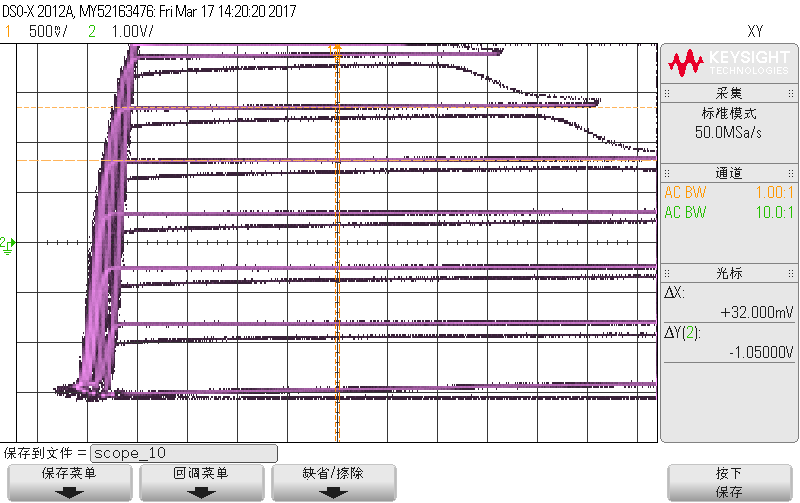
\includegraphics[width=\textwidth]{scope_10.png}
\caption{对$\beta$的测量}
\label{testBJT}
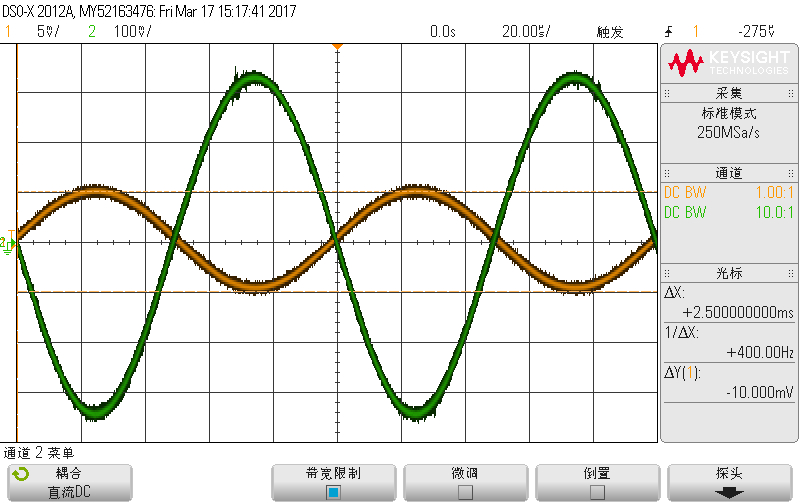
\includegraphics[width=\textwidth]{scope_14.png}
\caption{电路对波形的放大示意}
\label{exppic}
\end{figure}
\subsection{三极管频率特性的测试}
本实验中,对三极管的频率特性进行了细致的测试,先列出两种情况的最高频率和最低频率如表\ref{frec}所示

同时,如表\ref{tablef1},\ref{tablef2}所示,为三极管在两种状态下的辐频特性和相频特性,得到图\ref{bode1exp},\ref{bode2exp}的幅相特性(图中频率为分贝值)

限于篇幅,有关频域特性问题的进一步讨论在课程论文中阐述
\begin{table}
\centering
\caption{放大电路的工作最高频率和最低频率}
\label{frec}
\begin{tabular}{|c|c|c|}
\hline
\tabincell{c}{$I_{CQ}/\rm{mA}$}& \tabincell{c}{$f_L/\rm{kHz}$} & \tabincell{c}{$f_H/\rm{kHz}$}\\
\hline
1.00&0.105&280\\
\hline
2.00&0.170&170\\
\hline
\end{tabular}
\begin{multicols}{2}
\caption{$I_{CQ}=1\rm{mA}$时的辐频相频特性}
\label{tablef1}
\begin{tabular}{|c|c|c|}
\hline
\tabincell{c}{$f/\rm{Hz}$}& \tabincell{c}{$|\dot{A}|$} & \tabincell{c}{$\phi$}\\
\hline
$10^{0}$&0.9875&-89.28\\
\hline
$10^{0.5}$&2.1125&-93.8\\
\hline
$10^{1}$&5.2375&-97.2\\
\hline
$10^{1.5}$&14.2875&-111.82\\
\hline
$10^{2}$&32.125&-126.04\\
\hline
$10^{2.5}$&43.875&-157.61\\
\hline
$10^{3}$&47.875&-159.09\\
\hline
$10^{3.5}$&48.25&-166.23\\
\hline
$10^{4}$&48.375&-173.41\\
\hline
$10^{4.5}$&48.125&-180.17\\
\hline
$10^{5}$&45.000&-188.56\\
\hline
$10^{5.5}$&32.250&-223.5\\
\hline
$10^{6}$&12.6625&-270.5\\
\hline
$10^{6.5}$&4.25&---\\
\hline
$10^{7}$&1.325&---\\
\hline
\end{tabular}
\caption{$I_{CQ}=2\rm{mA}$时的辐频相频特性}
\label{tablef2}
\begin{tabular}{|c|c|c|}
\hline
\tabincell{c}{$f/\rm{Hz}$}& \tabincell{c}{$|\dot{A}|$} & \tabincell{c}{$\phi$}\\
\hline
$10^{0}$&0.5025&-59.04\\
\hline
$10^{0.5}$&1.925&-86.52\\
\hline
$10^{1}$&7.650&-94.68\\
\hline
$10^{1.5}$&16.100&-101.0\\
\hline
$10^{2}$&38.000&-124.09\\
\hline
$10^{2.5}$&62.5&-150.71\\
\hline
$10^{3}$&70.5&-167.60\\
\hline
$10^{3.5}$&72.5&-178.02\\
\hline
$10^{4}$&73.00&-183\\
\hline
$10^{4.5}$&72.00&-188.73\\
\hline
$10^{5}$&64.00&-206.03\\
\hline
$10^{5.5}$&36.00&-230.8\\
\hline
$10^{6}$&13.5&-263.2\\
\hline
$10^{6.5}$&4.5&---\\
\hline
$10^{7}$&1.6&---\\
\hline
\end{tabular}
\end{multicols}
\end{table}
\begin{figure}
\centering
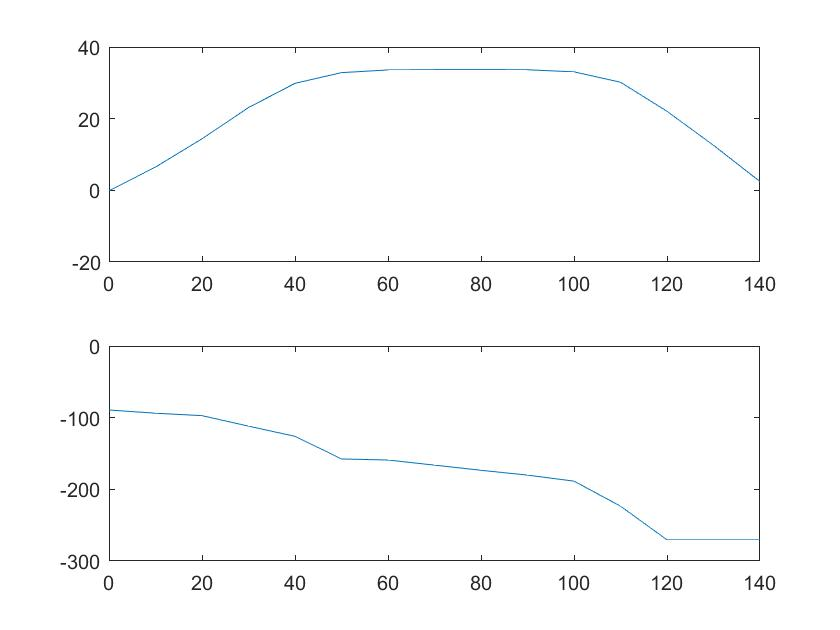
\includegraphics[width=\textwidth]{bode1exp.jpg}
\caption{$I_{CQ}=1\rm{mA}$,实验测得bode图}
\label{bode1exp}
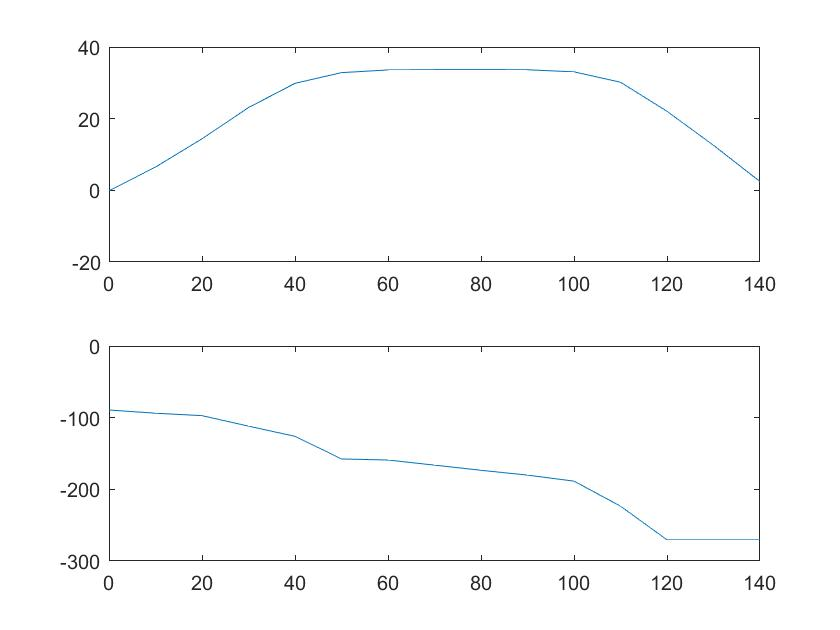
\includegraphics[width=\textwidth]{bode1exp.jpg}
\caption{$I_{CQ}=2\rm{mA}$,实验测得bode图}
\label{bode2exp}
\end{figure}
\section{实验总结}
\subsection{数据分析与比较}
三个实验中放大倍数、输入电阻和输出电阻值均较为吻合。选做任务和必做任务相比,减小了发射极电阻,以牺牲电压放大倍数为代价提高了电路的稳定性;输入电阻增大,输出电阻不变。
\subsection{电路故障与分析解决}
本次试验较为顺利,没有出现电路故障。
\subsection{发射极电阻对放大电路动态参数的影响}
增加发射极电阻使电路产生了交、直流负反馈,电压放大倍数降低,但增加了放大电路的稳定性,增大输入、输出电阻,使电路的通频带被展宽。
\subsection{从控制理论角度对放大电路的研究和矫正}
在实验室老师的指导下完成了这方向的进一步研究和课程论文的写作工作
\end{document}